\chapter{LaTeX-Grundlagen}\label{app:latex}

\LaTeX\ ist ein Softwaresystem, das Klartext entgegennimmt und ihn anschließend zu einem formatierten Dokument kompiliert. Das bedeutet, dass sich die Nutzerin bzw. der Nutzer hauptsächlich auf die Struktur konzentriert und Kapitel, Abschnitte, Unterabschnitte, Unter-Unterabschnitte, Absätze und Unterabsätze erstellt. Befehle beginnen mit einem Backslash ($\backslash$), und das Prozentzeichen (\%) bzw. das Tastenkürzel Strg + T dient zum Erstellen eines Kommentars. % Kommentar

\section{Literatur}
Literaturangaben sollten in die Datei \texttt{references.bib} eingefügt werden. Die meisten Online-Quellen erlauben den Export im BibTeX-Format; dabei ist jedoch darauf zu achten, dass die Angaben vollständig sind und im gleichen Format wie die übrigen Quellen vorliegen. Anschließend kann die Quelle mit dem Befehl \texttt{$\backslash$cite} (\ac{bzw} \texttt{$\backslash$autocite}) im Text zitiert werden.

\section{Gleichungen}

Ein großer Vorteil ist, dass Gleichungen leicht eingefügt werden können, wie in \autoref{eq:1}. Diese müssen in einer speziellen Mathematikumgebung gesetzt werden. Üblich sind \texttt{$\backslash$begin\{equation\}} und \texttt{$\backslash$end\{equation\}} für einzelne Gleichungen, \texttt{$\backslash$begin\{align\}} und \texttt{$\backslash$end\{align\}} für mehrere Gleichungen sowie Dollarzeichen für ein \$$mathematisches\ Ausdruck$\$ im Fließtext.

\begin{equation}
	\alpha = \frac{\beta^2}{\gamma}\label{eq:1}
\end{equation}

\begin{equation}
	\acs{force} = \ac{mass} \cdot \ac{acceleration}\label{eq:2}
\end{equation}


\section{Verweise}
Mit dem Befehl \texttt{$\backslash$label} kann nahezu alles im Dokument versehen werden, von Kapiteln und Abschnitten bis hin zu Gleichungen, Abbildungen oder Tabellen. \texttt{$\backslash$ref} (\ac{bzw} \texttt{$\backslash$autoref} wenn das Paket \texttt{$\backslash$hyperref} verwendet wird) erzeugt einen Verweis im Text, etwa auf \autoref{fig:graph}. Gleichungen werden in der Regel mit \texttt{$\backslash$eqref} referenziert.

\section{Gleitobjekte}
Abbildungen oder Tabellen werden als Gleitobjekte (engl. floats) bezeichnet, da sie nicht über eine Seite umbrochen werden können. Ihre Position wird automatisch in Abhängigkeit von ihrer Platzierung im Text und dem Positionsparameter in eckigen Klammern festgelegt, \ac{dh} \texttt{h, t, b, p} (für here, top, bottom, page). Die Umgebung wird wiederum mit den Befehlen \texttt{$\backslash$begin} und \texttt{$\backslash$end} erstellt. Abbildungen sollten, sofern geeignet, als Vektorgrafiken (\texttt{.eps}) eingefügt werden. Diagramme können auch mit dem Paket \texttt{pstricks} erstellt bzw. eingefügt werden.
Bildunterschriften für Abbildungen stehen unter dem Gleitobjekt, diejenigen für Tabellen darüber. Außerdem kann in spitzen Klammern eine Kurzfassung der Beschriftung angegeben werden, die dann im Abbildungs-/Tabellenverzeichnis erscheint.

\begin{figure}[ht]
	\centering
	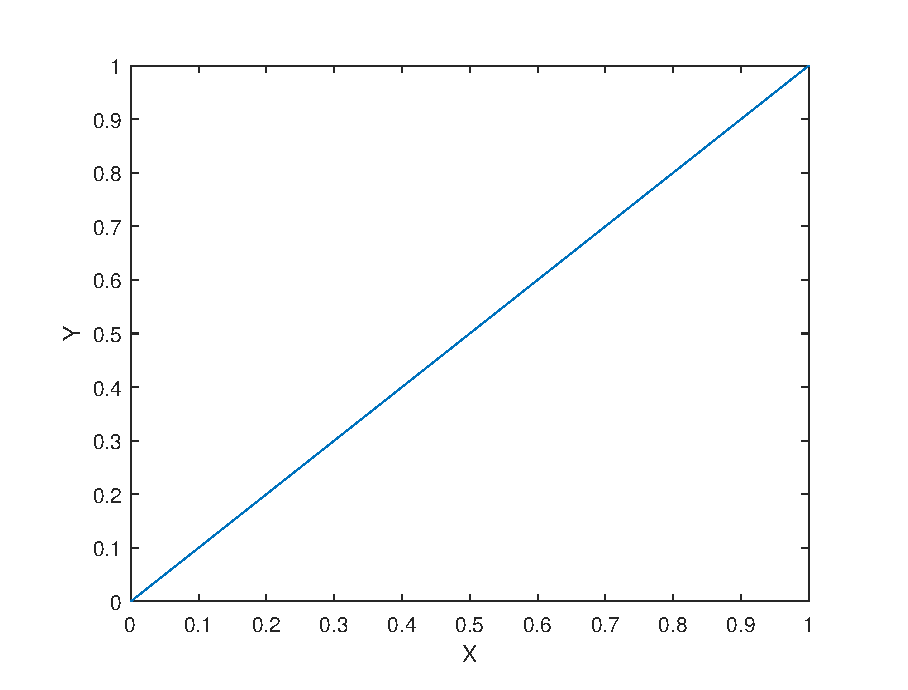
\includegraphics[width=0.75\textwidth]{figures/graph.eps}
	\caption[Graph]{Fügen Sie Abbildungen nach Möglichkeit als .eps-Dateien ein.}
	\label{fig:graph}
\end{figure}

\begin{table}[hpt]
	\centering
	\caption[Tabelle]{Tabelle}\label{tab:table}
	\begin{tabular}{c|cc}
		\hline
		& System 1 & System 2\\\hline
		Daten 1 & 0.1 & 0.2\\
		Daten 2 & 0.3 & 0.4\\\hline
	\end{tabular}
\end{table}

\section{Abkürzungen}
\acresetall % Alle Abkürzungen zurücksetzen, damit sie im Text erneut ausgeschrieben werden
Abkürzungen sind im Paket \texttt{acro} in der Datei \texttt{abbreviationsAndSymbols.tex} definiert. Sie können mit dem Befehl \texttt{$\backslash$ac} im Text verwendet werden, wobei die ausgeschriebene Form beim ersten Auftreten automatisch generiert wird. Es ist auch möglich, die Kurzform mit \texttt{$\backslash$acs} oder die Langform mit \texttt{$\backslash$acl} explizit zu verwenden. Weitere Informationen zum Paket \texttt{acro} finden Sie in der ausführlichen Dokumentation unter \url{https://ctan.org/pkg/acro?lang=en}.
Die definition der Größenzeichen und Einheiten erfolgt ebenfalls in \texttt{abbreviationsAndSymbols.tex} und kann mit dem Befehl \texttt{$\backslash$ac} im Text verwendet werden. Die korrekte darstellung von Einheiten erfolgt mit dem Paket \texttt{siunitx}.
Abkürzungen sowie Größenzeichen und Einheiten werden im Inhaltsverzeichnis unter den Kapiteln "Abkürzungen" bzw. "Formelsymbole" automatisch nach verwendung aufgeführt. Es ist wichtig, dass die Abkürzungen und Symbole in der Datei \texttt{abbreviationsAndSymbols.tex} sorgfältig definiert werden, damit sie korrekt im Text und in den Verzeichnissen dargestellt werden (siehe Beispiele in der Datei).

\section{Weitere Informationen}
Für weiterführende Informationen zu \LaTeX, etwa zu Befehlen für mathematische Symbole oder Konventionen beim Querverweisen, konsultieren Sie die Dokumentationen unter \url{https://en.wikibooks.org/wiki/LaTeX} und \url{https://overleaf.com/learn}. Die meisten Fragen zu speziellen Formatierungen in \LaTeX\ wurden zudem in einem der zahlreichen \LaTeX-Foren online bereits beantwortet.
```